\documentclass{article}
\usepackage[margin=1in]{geometry}
\usepackage{biblatex}
\usepackage{psfrag}
\usepackage{amsmath,amssymb,bbm,nicefrac,mathtools,lipsum, amsthm}
\usepackage{array}
\usepackage{latexsym}
\usepackage{graphicx}
\usepackage{textcomp}
\usepackage{framed}
\usepackage{lineno}
%\usepackage{tikz}
\usepackage{mathtext}
%\usetikzlibrary{shapes,arrows}
\usepackage{balance}
%\usepackage[nodisplayskipstretch]{setspace}
\usepackage{colortbl}
\usepackage{fancyhdr}
\usepackage{epstopdf}
\usepackage{float}
\usepackage{hyperref}
\usepackage{booktabs,tabularx}
\usepackage{anyfontsize}
\usepackage{authblk}
\usepackage{cleveref}
\usepackage{siunitx}
\usepackage{authblk}
\usepackage[width=13cm, justification=justified]{caption}
\usepackage{physics}
\usepackage{enumitem}
\usepackage{soul}
\usepackage[super]{nth}
\usepackage[ruled]{algorithm2e}
\usepackage[bottom,hang,flushmargin]{footmisc}
\usepackage{cancel}
\usepackage{optidef}
\usepackage{multirow}
\usepackage{subcaption}
\usepackage{bm}
\usepackage{xcolor}
\definecolor{grey}{rgb}{0.5, 0.5, 0.5}

% TikZ libraries
%\usetikzlibrary{positioning}

% Commands
\newcommand{\red}{\textcolor{red}}
\newcommand{\blue}{\textcolor{blue}}

\urlstyle{ttfamily}

\graphicspath{{./figures/}}

\date{\today}

\DeclareMathOperator*{\argmin}{arg\,min}

\setlength{\belowdisplayskip}{0pt} \setlength{\belowdisplayshortskip}{0pt}
\setlength{\abovedisplayskip}{0pt} \setlength{\abovedisplayshortskip}{0pt}

% Better looking tables
\renewcommand{\arraystretch}{1.2}

\fancyhf{} 
\renewcommand{\headrulewidth}{0pt}
\lfoot{E. Legrand}
\cfoot{Orientation Control in Space}
\rfoot{\thepage}
\pagestyle{fancy}

\addbibresource{references.bib}

\makeatother
\renewcommand*{\thefootnote}{\fnsymbol{footnote}}
\setcounter{footnote}{1}

\sisetup{per-mode=symbol}

\begin{document}
\begin{titlepage}
	\centering
	%\includegraphics[width=0.15\textwidth]{example-image-1x1}\par
	\vspace{2cm}
	{\scshape\large Delft University of Technology \par}
	\vspace{1cm}
	{\scshape\large SC42095 - Control Engineering\par}
	\vspace{3cm}
	\rule{\linewidth}{1.2pt}\\[0.5cm]
    {\huge\bfseries Orientation Control in Space\par}
	\vspace{0.5cm}
	\rule{\linewidth}{1.2pt}\\[0.5cm]
	\vspace{1.5cm}
	{\Large\itshape Emiel Legrand \footnote{4446100 -  \href{mailto:e.b.legrand@student.tudelft.nl}{\texttt{e.b.legrand@student.tudelft.nl}}} \par}
	\vfill

% Bottom of the page
	{\large \today\par}
	\vfill
\end{titlepage}

\renewcommand*{\thefootnote}{\arabic{footnote}}
\setcounter{footnote}{0}

\clearpage
\renewcommand{\thepage}{\roman{page}}% Roman numerals for page counter

\setcounter{page}{1}
\tableofcontents
\clearpage

\renewcommand{\thepage}{\arabic{page}}% Arabic numerals for page counter
\setcounter{page}{1}
\clearpage

\section{Introduction}
[Intro here]
\clearpage

\section{Continous-time PID controller}
\subsection{Analysis of the plant}
\label{sec:plant}
The transfer function of the plant is
\begin{equation}
    G(s) = \frac{s+20}{s\qty(s^2 + 24s + 144)}
    \label{eq:plant}
\end{equation}
Clearly, the system has two poles at $s = -12$ and one pole at the origin. There is one zero located at $s = -20$ (all on the real axis). A pole-zero map of the system is shown in \cref{fig:cont_plant_pzmap}. 
\begin{figure}[ht]
    \centering
    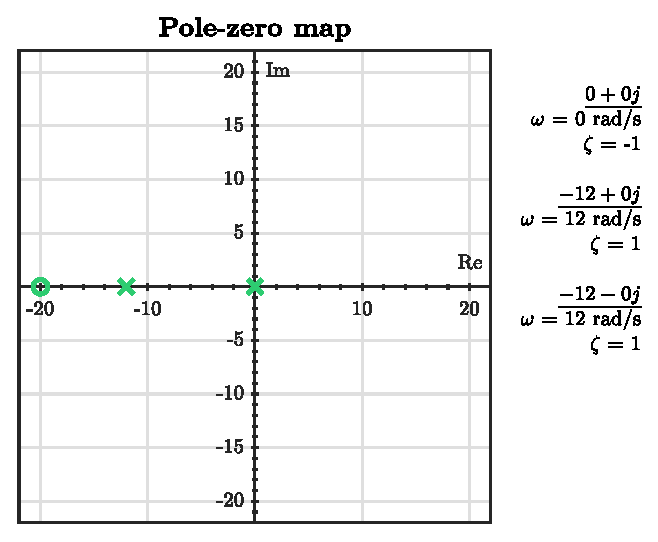
\includegraphics[]{media/q1/cont_plant_pzmap.eps}
    \caption{Pole-zero map of the continuous-time plant model. Clearly, the plant has only real, stable poles and zeros.}
    \label{fig:cont_plant_pzmap}
\end{figure}
From inspection of the poles and zeros, it can be concluded that the plant is \nth{3}-order, minimum phase and open-loop stable. Furthermore, because of the pole at $s = 0$, this is a so-called Type-I system. This means that the system is able to track a step reference with perfect steady-state accuracy. Looking at the frequency response function associated with \cref{eq:plant} shown in \cref{fig:cont_plant_bode}, a few additional remarks can be made:
\begin{itemize}
    \item Because the system is Type-I, it approaches $j\omega = 0$ with a slope of \SI{-20}{\decibel\per dec}.
    \item The stability margins of the system are ample: the phase margin is \ang{89.1} and the gain margin infinitely large since the system never crosses (although barely) the \ang{-180}-line. The system is therefore \textit{structurally} stable, i.e. the gain can be increased arbitrarily without causing the poles to venture into the right-half plane.
    \item Overall, the plant shows moderate gains around for low-frequencies and very strong attenuation of frequencies higher than those associated with the double pole at \SI{12}{\radian\per\second}.
\end{itemize}

\begin{figure}[ht]
    \centering
    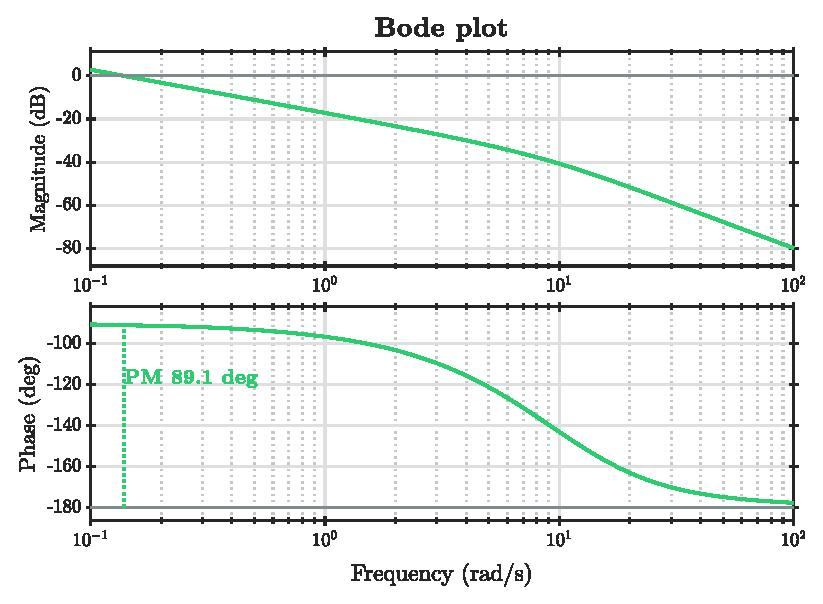
\includegraphics[]{media/q1/cont_plant_bode.eps}
    \caption{Bode plot of the plant. The stability margins are indicated on the plot (the phase margin is \ang{89.1}, the gain margin is infinite).}
    \label{fig:cont_plant_bode}
\end{figure}

\subsection{Set-point tracking\textnormal{\phantom{xxx}(Question 1)}}
\label{sec:continuoustracking}
First, a PID-controller has to be designed for reference-tracking. The following constraints are imposed on the design:
\begin{itemize}
    \item Minimal settling-time
    \item The response overshoot shall not exceed 5\%
    \item No steady-state error
\end{itemize}

\paragraph{Controller structure}
Because the system is Type-I, integral action will not be necessary to avoid steady-state tracking errors. Although the stability margins are very generous, adequate performance may be achieved purely by proportional control. However, due to the strict overshoot requirements and the desire to reduce the settling-time to an absolute minimum, more damping will likely be required in the form of one or two D-terms, resulting in a PD(D)-type controller.

\paragraph{Frequency-domain requirements}
The formerly stated requirements are specified in the time-domain. Because the controller design will be achieved by shaping the loop transfer function, it makes sense to translate these requirements to an (approximate) frequency-domain counterpart. Because analytical results only exist for \nth{2}-order plants, these results will only serve as an approximate target value. Some iteration using a simulation of the closed-loop step response will be inevitable to fine-tune the controller design.

As specified by \textcite{nise}, the following relations hold for a \nth{2}-order plant. First of all, the relation between the bandwidth of the closed-loop system and its settling time is:
\begin{equation}
    \omega_{BW} = \frac{4}{T_s\zeta}\sqrt{\qty(1 - 2\zeta^2)+\sqrt{4
    \zeta^4-4\zeta^2+2}}
    \label{eq:damping}
\end{equation}
Hence, to minimize the settling time one preferably has a damping ration $\zeta$ close to unity and maximise the $\omega_\text{BW}$, which in turn means that the cross-over frequency of the loop transfer function should be as large as possible. Furthermore, the overshoot of the system can be related to the damping ratio as follows:
\begin{equation}
\%\text{OS} = 100\times \exp(-\frac{\zeta \pi}{\sqrt{1-\zeta^2}})
\label{eq:overshoot}    
\end{equation}
This equation suggests that for an overshoot of 5\%, one should aim for $\zeta \approx 0.69$.
Since $\zeta$ is still not directly visible on the loop transfer Bode plot, there also exists a relation between the damping ratio and the phase margin $\phi_m$:
\begin{equation}
\phi_m = \tan[-1](\frac{2\zeta}{\sqrt{-2\zeta^2 + 1 + \sqrt{1 + 4\zeta^4}}})
\label{eq:settlingtime}    
\end{equation}
Based on the required $\zeta$, this yields a target for the phase margin of ca. \ang{64.2}.

\paragraph{Loop shaping}
The computed target phase margin suggests to start with pure proportional control and increase $K_p$ until the phase margin has decreased from \ang{89.1} to \ang{64.6}. \Cref{fig:cont_plant_bode} hints that the new crossover frequency should then be at \SI{4}{\radian\per\second}, which means the gain can be increased by \SI{29.9}{\decibel}. This simple step already results in a dramatic increase in the settling time from \SI{32.7}{\second} (no compensation) to \SI{1.04}{\second}. 

The overshoot for this controller is only 4.7\%, which is not quite limiting. As such, there is some more room to increase the gain further to 31.7, which results in a very marginal reduction of the settling time. Now, the limit of simple proportional control has been attained: in order to speed the response up even further, more damping (i.e. phase lead) must be added at the appropriate frequencies in order to observe the overshoot limit.

A realizable PD-controller has the following transfer function:
\begin{equation}
K_p \qty(1 + \frac{sT_d}{1 + sT_d/N}) = K_p\frac{1 + T_d(N+1)s/N}{1 + sT_d/N}
\label{eq:leadcomp}
\end{equation}
which is essentially the same as a lead-compensator with a pole far into the left-half plane ($N \gg 1$). The choice of $N$ determines the second corner frequency and is dependent on the physical implementation of the system and the actuators, since it will determine noise amplification and the initial jump in the controller effort. \textcite{keviczky} recommend this value between 4 and 6 during controller design, after which it can be retuned after testing with the physical plant. Hence, for the controller design, a value of $N=5$ was chosen. The choice of $N$ places an irrevocable limit on the maximum attainable phase contribution by the PI controller, as given by the following equation\footnote{The relations from \textcite{ogata} are based on a different parameterization of the compensator, but they are equivalent to those mentioned in this report.}: \cite{ogata}
\begin{equation}
\phi_\text{max} = \sin[-1](\frac{N}{N + 2}) \approx \ang{45}
\label{eq:maxphi}
\end{equation}
As mentioned before, the maximum phase contribution of the lead contribution occurs at the geometric mean of the pole and zero frequencie: \cite{ogata}
\begin{equation}
    \omega_{\phi_\text{max}} = \frac{N}{T_d\sqrt{N+1}}
    \label{eq:omegamaxphi}
\end{equation}
Using \crefrange{eq:maxphi}{eq:omegamaxphi}, the maximum phase contribution was placed at the highest frequency where the plant could still have the target phase margin of \ang{64.4} (i.e. the frequency at which the plant has a phase of $\ang{180} - \ang{64.4}  - \ang{45}$). This is shown as iteration \#3 in \cref{tab:loopshaping1}. In order to obtain the desired performance, the proportional gain $K_p$ must be adjusted accordingly. The result is iteration \#4 in \cref{tab:loopshaping1}; the settling time shows a substantial reduction of \%65 to \SI{0.39}{\second}. Finally, the controller was tuned a little more: in order to achieve minimal settling time, the response must be well-damped as illustrated by \cref{eq:settlingtime}. The controller was therefore retuned to have a higher phase margin (\ang{70}) --- from \cref{fig:cont_controllers_step} it is clear that this iteration has much better damping and a better settling time.
\begin{figure}
    \centering
    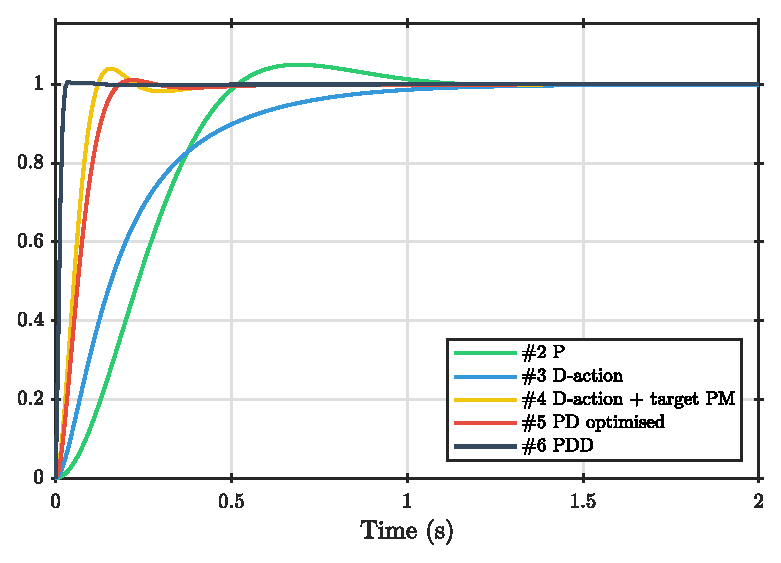
\includegraphics[]{media/q1/pd_controllers_step.eps}
    \caption{}
    \label{fig:cont_controllers_step}
\end{figure}
At this point, the limits of the PD-controller architecture are reached, due to the limited phase contribution given by \cref{eq:maxphi}, sufficient phase margin can only be guaranteed up to a certain frequency. 

Using yet another D-term the phase contribution can be increased even more; the result is a PDD-controller:
\begin{equation}
K_p \qty(1 + \frac{sT_{d_1}}{1 + sT_{d_1}/N})\qty(1 + \frac{sT_{d_2}}{1 + sT_{d_2}/N})
\label{eq:pdd}
\end{equation}
The idea behind the tuning process of these terms was to extend the region with sufficient phase towards higher frequencies without creating excessive `bumps' in the phase curve to obtain an even response. To do so, one lead compensator was placed to have its $\phi_\text{max}$ at about the same frequency as the previous one, while the other one was placed at a frequency about five times higher. The resulting phase and magnitude curves are, together with the previous iterations, displayed in \cref{fig:cont_controllers_bode}. Again, to achieve sufficient damping, the proportional gain was adjusted accordingly for a similar phase margin as iteration \#5, ca. \ang{71}. This final iteration results in a tenfold reduction of the settling time to \SI{0.0251}{\second}.
\begin{figure}[ht]
    \centering
    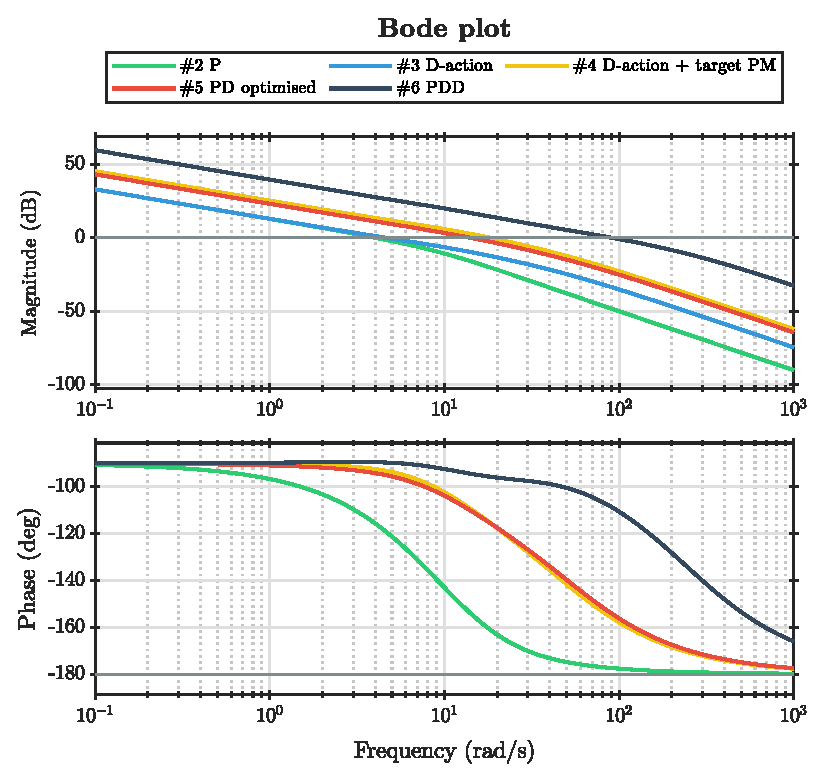
\includegraphics[]{media/q1/pd_controllers_bode.eps}
    \caption{}
    \label{fig:cont_controllers_bode}
\end{figure}
The final PDD controller is then:
$$ 
\begin{aligned}
C(s) &= 675.84\qty(1 + \frac{0.1021s}{1 + s0.1021/5})
            \qty(1 + \frac{0.0204s}{1 + s0.0204/5})\\
     &= \frac{50.69 s^2 + 2483 s + 16896}{0.002083 s^2 + 0.6124 s + 25}
\end{aligned}
$$
\begin{table}[ht]
    \centering
    \caption{Overview of the loop shaping process of the reference tracking controller.}
    \label{tab:loopshaping1}
    \begin{tabular}{ccccccc}
        \toprule
            \# & $K_p$ & $T_{d_1}$ & $T_{d_2}$ & $\phi_m$ (deg) & \%OS & $T_s (\si{\second})$ \\
        \midrule
            0 & 1 & 0 & 0 & 89.1 &  0 & 32.7\\ 
            1 & 31.14 &        0 &        0 &  64.6 &   4.7 &  1.04\\ 
            2 & 31.71 &        0 &        0 &  64.2 &     5 &  1.03\\ 
            3 & 31.71 &    0.112 &        0 &  86.8 &     0 &  1.08\\ 
            4 & 130.8 &    0.112 &        0 &  64.7 &     4 & 0.387\\ 
            5 & 102.4 &    0.102 &        0 &    70 &   1.1 & 0.233\\ 
            6 & 675.8 &    0.102 &   0.0204 &  71.3 &  0.71 & 0.0267\\ 
        \bottomrule
    \end{tabular}
\end{table}

\subsection{Disturbance rejection\textnormal{\phantom{xxx}(Question 2)}}
\label{sec:continuousdisturbance}
In this section, another contoller will be designed specifically for the rejection of a load disturbance $q$ that acts on the control input in the form of a step input. The following requirements are to be fullfilled:
\begin{itemize}
    \item Minimal amplitude of the output as a result of the disturbance.
    \item Minimal duration of the disturbance.
    \item The disturbance shall cause no offset in the response.
\end{itemize}
\paragraph{Controller structure}
The closed-loop transfer function from the load disturbance $q$ to the output $y$ is straightforward to determine:
\begin{equation}
    G_q(s) = \frac{G(s)}{1 + G(s)K(s)} = G(s)S(s)\qq{with}S = \frac{1}{1 + G(s)K(s)}
    \label{eq:disttf}
\end{equation}
where $S(s)$ is the so-called sensitivity transfer function of the closed-loop. Clearly, the sensitivity function will have the poles of the loop transfer function as zeros. \Cref{sec:plant} already mentions that the system is Type-I. Therefore, the sensitivity function must have a \textit{zero} at $s = 0$. As such, in the transfer function $G_d(s)$ the zero from $S$ and the pole from $G_d$ cancel. In order to meet the requirements and have no steady-state offset in the response due to the load disturbance, the final value theorem states that $\lim_{s\to 0} sG_d(s)\frac{1}{s}$. As such, $G_d(s)$ must have a zero at $s = 0$ (which of course should not be cancelled). This can be achieved by placing an extra pole in the controller at $s = 0$; in other words: integral action will be instrumental to eliminate steady-state offset as a result of the load disturbance. Hence, the controller will be of the type PI(DD).

\paragraph{Frequency-domain requirements}
Ideally, the transfer function from the disturbance $q$ to the output $y$ is no-pass (i.e. none of the frequency components in the disturbance persist to the output). Of course, this is not achievable. However, from inspection of \cref{eq:disttf} it is clear that for frequencies where the loop gain $\abs{G(s)K(s)}$ is high will $G_d(s)$ will show proper damping. Hence, high proportional gain and lag compensation (i.e. high gain contribution at lower frequencies) will decrease the settling time of the output after the introduction of the step load disturbance. The plant itself is low-pass with a very low crossover frequency; hence one can expected that high controller gain will be required to reject the disturbance quickly. Besides, the aforementioned requirements will likely contradict with those of the previous controller: where for the tracking case a generous phase margin reduced the settling time, higher damping in the case of disturbance rejection will jeopardise the controller's ability to amplify frequency components to a sufficient extent which in turn would mitigate the effect of the load disturbance on the output.

\paragraph{Loop shaping}
It is already known that a PI-controller structure will be inevitable to obey the imposed constraints. As such, the limits of this controller type will be explored first after which the potential extension to a PID(D) type controller can be investigated. The PI-controller has the transfer function
\begin{equation}
    K_p\qty(1 + \frac{1}{T_is})
\end{equation}
which has a pole at $s = 0$ and a zero at $s = -1/T_i$. The zero determines the second corner frequency of the controller, and therefore up to which frequency the amplification occurs. Simultaneously, the PI controller will introduce a destabilising phase lag for lower frequencies, also determined by the position of this zero.

Because the proportional gain $K_p$ does not affect the phase curve of the system, the maximum attainable phase margin (i.e. where the phase curve is maximal) is purely determined by the choice of $T_i$. A higher phase margin gives better damping of oscillatory respones but also means that $T_i$ must be higher, which decreases the amplification of the lower frequencies with a deterioration of the settling time as a result (the slower frequencies will take longer to be rejected by the system). Oscillations in the response may on the other hand also slow down the time it takes for the output to return to zero, so a compromise has to be found. \Cref{fig:pm_comparison} shows a comparison of three values for the phase margin: for each of these, $T_i$ was tuned to make sure that the maximum attainable phase margin would be equal to a set value (\ang{35}, \ang{41} and \ang{45}), after which $K_p$ was tuned to set the crossover frequency at the correct value. Clearly, the settling time is lowest for $\phi_m = \ang{40}$, so this value was used as an approximate tuning value for $T_i$. 
\begin{figure}
    \centering
    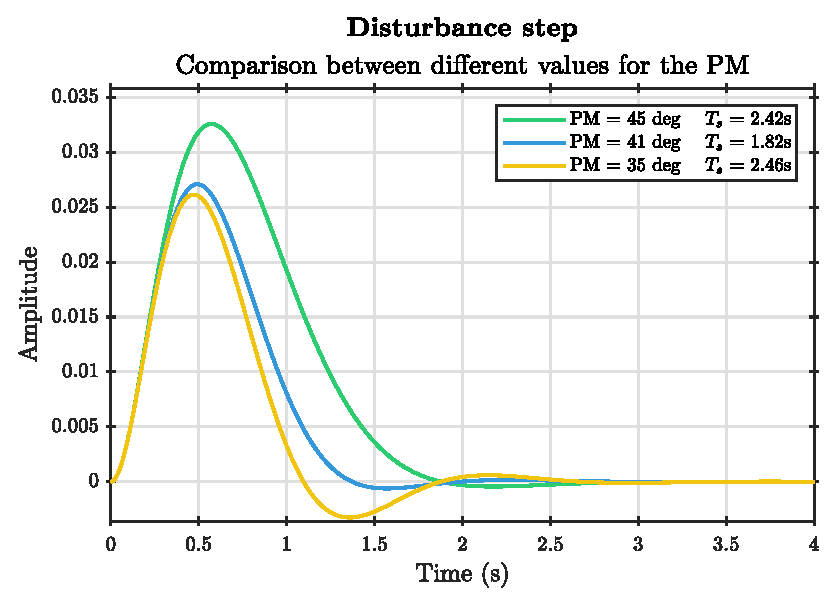
\includegraphics[]{media/q2/pi_pm_comparison.eps}
    \caption{}
    \label{fig:pm_comparison}
\end{figure}

It has to be noted that the two first requirements are conflicting, since both the peak amplitude and the settling time must be minimised, without a quantifiable priority of one over the other. Indeed, in \cref{fig:pm_comparison} one can see that for $\phi_m = \ang{35}$, the peak value is slightly lower. However, because the relative difference in the peak value is relatively low compared to the difference in settling time, $\phi_m = \ang{40}$ is said to show the `better' performance.

At this point, no better performance (in terms of settling time) can be achieved by using the PI controller structure: to lower the settling time $T_i$ must be decreased to amplify the lower frequencies to a greater extent. However, this creates two issues: firstly, the phase curve will at some point cross the \ang{-180} line, which will render the system immediately unstable: the gain will cross-over at a higher frequency. Decreasing the gain is not an option since it will yield a dramatic increase of the peak amplitude. Secondly, as illustrated by \cref{fig:pm_comparison} the smaller phase margin results in badly damped oscillatory artefacts in the response even before the point of instability is reached. Therefore, one must resort to D-action to add phase advance at these higher frequencies to keep sufficient phase margin and prevent the phase from crossing over. As in \cref{sec:continuoustracking}, a realizable D-term as described by \cref{eq:leadcomp} will be used with $N = 5$. 

\sisetup{scientific-notation=engineering}
The loop shaping process for the PID controller was as the following: first, the $T_d$ term was chosen such that the maximum phase contribution occurs at a frequency where the phase of the previous controller was about \ang{-170}. This left about \ang{15} of excess phase (that is on top of the `ideal' \ang{40}), which could then be absorbed by decreasing $T_i$ further. In the subsequent tuning process, the purpose was always to decrease $T_i$ as much as possible while keeping sufficient phase margin and prevent the phase from crossing the \ang{-180} line. Finally, $K_p$ was chosen to set the cross-over frequency at the peak of the phase curve. The best PID controller turned out to achieve a settling time of \SI{0.70}{\second} and a peak amplitude of \num{0.00285}.

The final performance of the PID controller begs the question whether additional performance improvements could be made by adding additional gain with another D-term, just like in \cref{sec:continuoustracking}. The tuning of this PIDD controller was straightforward: one of the lead compensator was kept at a lower frequency to keep the phase from dipping under the \ang{-180} line, while the other lead compensator was placed at a frequency of about \SI{140}{\radian\per\second} to be able to have the desired phase margin at higher frequencies. After tuning, the resulting PIDD controller resulted in a settling time of \SI{0.4381}{\second} and a peak amplitude of \num{7.177e-05}. Although this performance is of course very nice, one can observe from \cref{fig:q2_bode_comparison} that the result from the PIDD is not desirable as for the other controllers, in the sense that there is a large phase contribution at lower frequencies and therefore inevitably also a decrease in gain amplification. This has as the result that the speed up of the settling time is `only' \%50. The problem is that due to the impending instability, the phase contribution could not be placed at higher frequencies to make it more limiting. One could therefore wonder whether the added complexity of the PIDD controller is worth the modest advancement in performance. The final controller has the following transfer function:
$$ 
\begin{aligned}
C(s) &= 4464\qty(1 + \frac{1}{0.05s})
           \qty(1 + \frac{0.017s}{1 + s0.017/5})
           \qty(1 + \frac{0.051s}{1 + s0.051/5})\\
     &= \frac{6.975 s^3 + 595.1 s^2 + \num{1.469e04} s + 111600}{\num{4.34e-05} s^3 + 0.01701 s^2 + 1.25 s}
\end{aligned}
$$


\begin{figure}[ht]
    \centering
    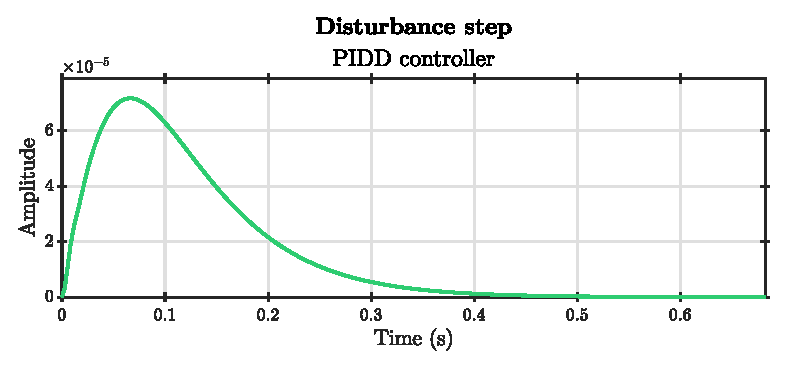
\includegraphics[]{media/q2/pidd_response.eps}
    \caption{}
    \label{fig:q2_pidd_response}
\end{figure}
\begin{figure}[ht]
    \centering
    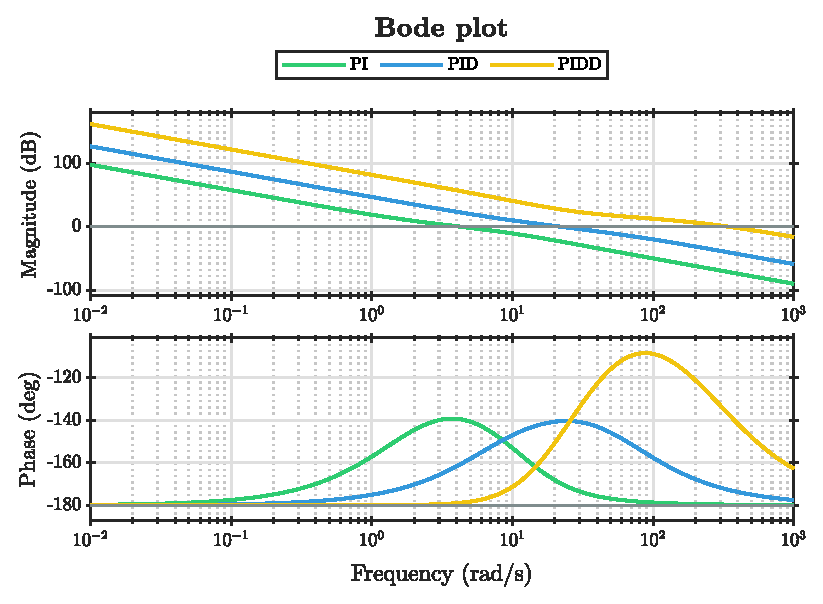
\includegraphics[]{media/q2/pi_bode_comparison.eps}
    \caption{}
    \label{fig:q2_bode_comparison}
\end{figure}
\clearpage

\section{Discretisation of the problem}
\subsection{Discretisation of the plant \textnormal{\phantom{xxx}(Question 3)}}
The transfer function of the plant (\cref{eq:plant}), has the state-space realization in the following canonical form:
\begin{equation}
    \begin{aligned}
        \dv{x}{t} &= \mqty(0 & 1 & 0 \\ 0 & 0 & 1 \\ 0 & -144 & -24)x + \mqty(0 \\ 1 \\ -4)u\\
        y &= \mqty(1 & 0 & 0)x
    \end{aligned}
\end{equation}
It is known that the output of the system represents the orientation of the space station. From the state space description, it is therefore clear that the first state must also be equal to this orientation. Then, from the first state-space equation it is clear that $\dv{x_1}{t} = x_2$; which means that $x_2$ represents the angular velocity associated with the orientation of the spacecraft. Again, $\dv{x_2}{t} = x_3 + u$. Clearly, $u$ acts as a torque on the change in angular velocity; $x_3$ must therefore represent the angular acceleration. The third equation states that $\dv{x_3}{t} = -144x_2 - 24x_3 -4u$. It is not entirely evident what this equation represents, but it introduces some coupling between the angular velocity and the angular acceleration of the system. Therefore, one might guess that this equation represent some gyroscopic effect that is present in the rotational dynamics of the system --- a common way to adjust the attitude of spacecraft is by means of so-called Control Moment Gyroscopes.

\paragraph{Discretisation of the plant}
To find a discrete-time state-space representation of the plant a suitable sampling period $h$ has to be chosen. \textcite[300]{astrom} provides the rule for open-loop systems that
$$ \omega_ch \approx 0.15 \text{ to } 0.5$$
where $\omega_c$ is the crossover frequency of the open loop system. Based on this rule, a sampling period of $h = \SI{1.08}{\second}$ was chosen; which is rather low, but so it the closed-loop uncompensated step response of the plant. Using the zero-order hold method, the resulting discrete-time state-space model is:
\begin{equation}
    \begin{gathered}
        x(k+1) = \Phi x(k) + \Gamma u(k) \qquad y(k) = Cx(k) + Du(k)\\
        \Phi = 
        \begin{pmatrix}   
            1        &           0       &            0\\
            0.166663739616237  &  0.000032777038157 &  -0.000365153653910\\
            0.006944216826124 & 0.000002535789263  & -0.000028081904161 \\
        \end{pmatrix}\\
        \Gamma = \begin{pmatrix}
               1.080177590517217 \\
                0.159196525309621 \\
                 0.006343846186812\\ 
        \end{pmatrix}\quad C = \mqty(0 & 1 & -4) \quad D = 0
    \end{gathered}
\end{equation}

\subsection{Discretisation of the controllers \textnormal{\phantom{xxx}(Question 4)}}
Now, both the controllers from \cref{sec:continuoustracking,sec:continuousdisturbance} and the plant are discretised separately, after which a closed loop response simulation is performed. Again, another rule of thumb is used from \textcite[317]{astrom} for PID-type controllers:
$$ \frac{hN}{T_d} \approx 0.2 \text{ to } 0.6$$
Of course, the controller designs were of type PIDD so some care had to be taken when using this method.

\paragraph{Tracking controller}
The tracking controller was discretised using the Tustin approximation while the plant was discretised using the zero-order hold method (both with identical sampling period). The sampling period was computed using the aforementioned rule with the largest of the two $T_d$'s. The resulting sampling time was increased slightly more to obtain also a reasonable number of samples per rise time. The sampling time used was $h = \SI{0.0014}{\second}$. The resulting simulation is shown in \cref{fig:q4_dt_tracking}; the discretised controller shows comparable performance with slightly higher overshoot and settling time.
\begin{figure}[ht]
    \centering
    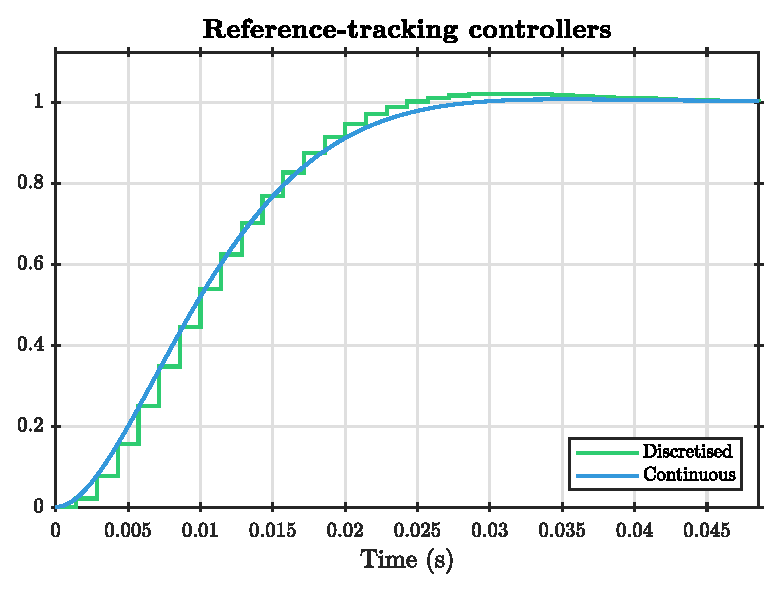
\includegraphics[]{media/q4/dt_tracking.eps}
    \caption{}
    \label{fig:q4_dt_tracking}
\end{figure}

\begin{figure}[ht]
    \centering
    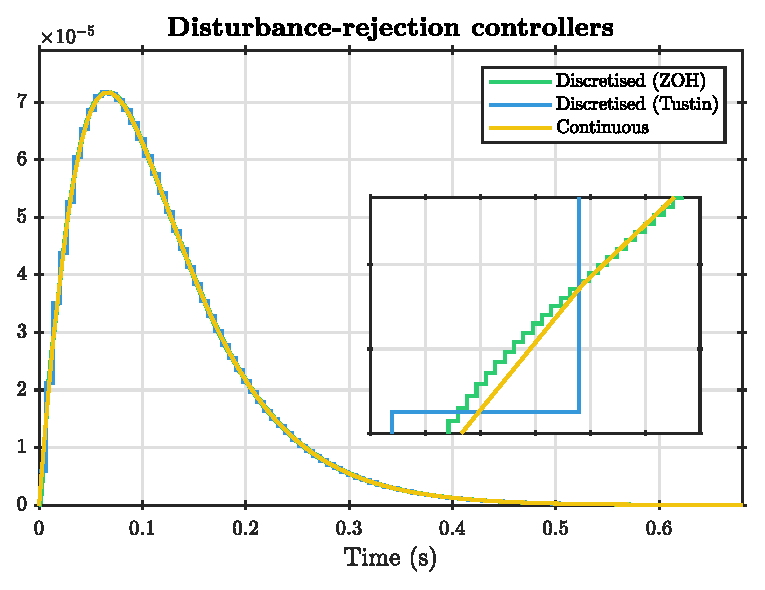
\includegraphics[]{media/q4/dt_distrej.eps}
    \caption{}
    \label{fig:q4_dt_distrej}
\end{figure}
\paragraph{Disturbance rejection controller}
Like the tracking controller, sampling period was based on the largest of the two $T_d$'s of the PIDD controller. This resulted in a sampling time of $h = \SI{3.4021e-04}{\second}$. However, the time constant of a step response is several orders of magnitude larger; so a larger sampling period may also be suitable to capture the same response. The meager stability margins of this controller did not allow to discretise the plant with zero-order hold for this larger sampling period due to excessive warping of the phase curve. Hence, the Tustin approximation was used for both the plant and the controller with a sampling time 25 times larger then the one used for the zero-order hold method. 

\Cref{fig:q4_dt_distrej} shows a comparison between the three methods: the continuous plant and controller, the plant discretised with ZOH and the controller with Tustin using the small $h$, and both discretised with Tustin using a larger sampling period. From the global perspective the first two responses are virtually indistinguishable (note the close-up view), so the Tustin approxmation definitely allows for a more reasonable sampling time while still capturing the system dynamics.
\clearpage

\section{State-space approach for controller design}
In this section, the controller design will be approached from a state-space perspective. First, a full-information state feedback controller will be designed for a servo problem in \cref{sec:ss_full}. Then, the assumption of full-information will be dropped; an observer will also be designed using pole-placement to provide the state information; this is discussed in \cref{sec:ss_output}. Finally, a linear quadratic regulator (LQR) solution is developed in \cref{sec:ss_lqr}.

\subsection{Full-information feedback using pole-placement\textnormal{\phantom{xxx}(Question 5)}}
\label{sec:ss_full}
In order to apply full-information feedback, information about all the states must be available. Using a feedback law $u = -Lx$ where $L$ is a vector to be designed to obtain the desired closed-loop behaviour. \Cref{fig:q5_block_statefeedback} visualises the process of state feedback in a block diagram for a servo problem. Please note that a feedforward gain $L_c$ is included as well which acts on the reference signal $r$; its purpose is to adjust the DC gain of the system to remove the steady-state error --- this matter will be discussed as well.
\begin{figure}[ht]
    \centering
    \includegraphics[scale=1.1]{media/q5/block_statefeedback-01.eps}
    \caption{}
    \label{fig:q5_block_statefeedback}
\end{figure}
The closed-loop state-space system in \cref{fig:q5_block_statefeedback}  (the feedthrough $D$ is assumed to be absent):
\begin{equation}
    \begin{aligned}
        x(k+1) &= \qty(\Phi - \Gamma L)x(k) + \Gamma L_c r(k)\\
        y(k) &= Cx(k)\\
    \end{aligned}
\end{equation}
According to the pole-placement theorem, the all poles of the system can be moved to any location of choice, provided that the system is reachable. Because the $\Phi$ matrix is invertible (this is always the case for sampled continuous-time systems, which cannot have a pole at $s = -\infty$), controllability and reachability are equivalent statements for this system. The reachability condition can be checked using the rank of the controllability matrix:
$$ W_c = \mqty(\Gamma & \Phi \Gamma & \cdots & \Phi^{n-1}\Gamma)$$
The system is reachable if and only if $\mathrm{rank}(W_c) = n$ ($n$ is the number of states), which is indeed the case for this system. As such, one can move all the poles to arbitrary locations using state-feedback.

\paragraph{Selection of the pole locations} Obviously, the selection of the closed-loop poles will be of major influence on the behaviour of the system. Therefore, it is important to choose them wisely. For the controller design, these locations where picked in the $s$-plane for continous-time systems, after which they are mapped to the $z$-plane for discrete-time systems using the relation:
$$ p_z = \exp(hp_s)$$
where $h$ is the sampling period, $p_z$ the pole location in the $z$-plane and $p_s$ the pole location in the $s$-plane. In the $s$-plane, the characteristics of the poles are very straightforward to compute:
$$ \omega = \abs{p_s} \qquad \zeta = -\frac{\Re{p_s}}{\abs{p_s}}$$
The general idea is to choose a dominant pole pair that will induce a second-order response with the desired $\zeta$ and $\omega$, and place the other pole(s) at a faster location; the result will then be approximately equal to the `design' response because the other modes will die out much quicker.
\sisetup{scientific-notation=false}
Using \cref{eq:overshoot,eq:damping}, the desired damping ratio can be computed based on the overshoot requirement. From the tuning of the PID controllers in \cref{sec:continuoustracking,sec:continuousdisturbance} it is already known that the maximum imposed overshoot limit is not desired for minimum settling time; rather, the overshoot should be limited to 1\% to keep the system immediately inside the `settling band' of $\pm 1\%$. Using these relations, one can find that the desired $\zeta = 0.83$. To have minimal settling time, $\omega$ should be as large as possible. However, this will also directly influence the distance over which the poles have to be moved and therefore the required control action. The settling time can, for second-order systems, be related to $\zeta$ and $\omega$ with the following expression (for continuous-time systems): \cite{nise}
$$ T_s = \frac{\ln(0.01\times\sqrt{1 - \zeta^2})}{\zeta\omega}$$
For the computed $\zeta$, an $\omega$ of \SI{25}{\radian\per\second} would yield a settling time of \SI{0.25}{\second}, comparable to the PD controller from \cref{sec:continuoustracking}. The remaining pole was placed at 30\% larger from the origin (because this is only a single pole, it must necessarily be on the real axis).
Hence, the resulting poles were placed in the at $-16.5 \pm 8.3j, -26 + 0j$. A value of $h = \SI{0.0192}{\second}$ was chosen for the sampling period, based on the time constant of the fastest pole.

Because state feedback leaves the zeros and gain of the system unaffected, the magnitude of its DC-gain cannot be influenced arbitrarily. Therefore, to avoid steady-state errors, the feedforward gain $L_c$ was chosen as the inverse of the steady-state gain of the closed-loop system. This will be treated in greater detail in \cref{sec:q12}.
\begin{figure}[ht]
    \centering
    \includegraphics{media/q5/dt_step.eps}
    \caption{}
    \label{fig:q5_step}
\end{figure}
Using the desired pole locations mapped to the $z$-plane, the feedback gain $L$ can be determined using the \textsc{Matlab}-command \texttt{place}. \Cref{fig:q5_step} also shows the response from some other pole locations; faster and slower, and with more or less damping. The response resulting from the discussed design process is also shown. \Cref{fig:cont_plant_pzmap} shows all the corresponding pole and zero locations in the $z$-plane; clearly the zeros remain in place regardless of the pole-placement controller design.
\begin{figure}[ht]
    \centering
    \includegraphics{media/q5/dt_pzmap.eps}
    \caption{}
    \label{fig:q5_pzmap}
\end{figure}

\subsection{Output feedback using pole-placement\textnormal{\phantom{xxx}(Question 6)}}
\label{sec:ss_output}
\subsubsection{Servo problem}
Now, it will no longer be assumed that all the states are known, but that the controller can only see the output of the system. To apply state feedback, the controller must include an observer that provides an estimate of the current state. \Cref{fig:q6_block_servo} shows how the plant and the controller are connected. To do so, the \textsc{Matlab} command \texttt{lft} (linear fractional transformation) was used.
\begin{figure}[ht]
    \centering
    \includegraphics[scale=1.3]{media/q6/block_outputfeedback-02.eps}
    \caption{}
    \label{fig:q6_block_servo}
\end{figure}
From \cref{fig:q6_block_servo}, it is straightforward to find the corresponding state-space models.
\begin{equation}
    \text{\textsc{Plant}}\qquad
    \begin{aligned}
        x(k+1) &= \Phi x(k) + \mqty(0&\Gamma)\mqty(r(k)\\u(k))\\
        \mqty(y(k)\\u(k)\\y(k)\\r(k)) &= \mqty(C\\0\\C\\0)x(k) + \mqty(0&0\\0&1\\0&0\\1&0) \mqty(r(k)\\u(k))
    \end{aligned}
\end{equation}
\phantom{x}
\begin{equation}
    \text{\textsc{Controller}}\qquad
    \begin{aligned}
        \hat{x}(k+1) =& (\Phi - KC)\hat{x}(k) + \mqty(\Gamma&K&0)\mqty(u(k)\\y(k)\\r(k))\\
        u(k) =& -L\hat{x}(k) + \mqty(0&0&L_c)\mqty(u(k)\\y(k)\\r(k))
    \end{aligned}
\end{equation}
The same pole locations were chosen as those designed in \cref{sec:ss_full} to obtain the state feedback gain $L$. It is common practice to place the observer poles faster than the controller, such that the state estimation error will decay faster to zero. The rationale behind this is perspicuous: it does not make sense to apply a state feedback law based on a state estimation that is way off. Therefore, the observer poles were chosen to be a factor 1.3 times the state feedback poles (in the $s$-plane). Translated to the $z$-plane, this resulted in:
$$0.6473 \pm 0.1370j \quad  0.5220$$
Again, the feedforward gain $L_c$ was used to eliminate the steady-state error; its computation will be discussed in \cref{sec:q12}. The resulting closed-loop system was simulated with a step reference input and the state estimates initialised at $\hat{x}_0 = \mqty(-20 & 30 & 50)$. The result is shown in \cref{fig:q6_output_servo}; both the output and the state estimation error are displayed. The state error decays to zero faster than the output attains it final value due to the faster observer poles. Also, there is only a marginal difference between the output feedback controller and the full information case from \cref{sec:ss_full}.
\begin{figure}[ht!]
    \centering
    \includegraphics[]{media/q6/output_servo.eps}
    \caption{}
    \label{fig:q6_output_servo}
\end{figure}

\subsubsection{Disturbance rejection}
Now, the output feedback controller will be used to reject a step load disturbance. Because the disturbance is not directly measurable and also not controllable by $u$, the controller must be equipped with an observer of the disturbance; only then will it have the ability to reject it succesfully. Since a step disturbance is assumed, the disturbance model simply reads:
                                $$v(k + 1) = v(k)$$
in combination with an initial condition $v_0$ (for the unit step disturbance, $v_0 = 1$). To turn this model into an observer, the mismatch between the plant output and the estimated output will be fed as an input to the observer, multiplied by a gain $K_w$. Finally, the output of the controller $u(k)$ is based on the feedback law:
                                $$u(k) = -L\hat{x}(k) - \hat{v}(k)$$
which means that the state feedback law is applied on the state estimate, after which the disturbance estimate is subtracted. To build this system, the \textsc{Matlab} command \texttt{lft} was used in a similar fashion as before. \Cref{fig:q6_block_distrej} shows the layout of the (generalised) plant and controller.
\begin{figure}[ht!]
    \centering
    \includegraphics[scale=1.3]{media/q6/block_distrej-03.eps}
    \caption{}
    \label{fig:q6_block_distrej}
\end{figure}
From \cref{fig:q6_block_distrej}, the state-space models of the plant and controller can be readily derived.
\begin{equation}
    \text{\textsc{Plant}}\qquad
    \begin{aligned}
        x(k+1) =& \Phi x(k) + \mqty(\Gamma&\Gamma)\mqty(v(k)\\u(k))\\
        \mqty(y(k)\\u(k)\\y(k)) =& \mqty(C\\0\\C)x(k) + \mqty(0&0\\0&1\\0&0)\mqty(v(k)\\u(k))\\ 
    \end{aligned}
\end{equation}
\phantom{x}
\begin{equation}
    \text{\textsc{Controller}}\qquad
    \begin{aligned}
        \mqty(\hat{x}(k)\\\hat{v}(k)) =& \mqty(\Phi-KC & \Gamma\\-K_wC&1)\mqty(\hat{x}(k)\\\hat{v}(k)) + \mqty(\Gamma&K\\0&K_\omega)\mqty(u(k)\\y(k))\\
        u(k) =& \mqty(-L&-1)\mqty(\hat{x}(k)\\\hat{v}(k))
    \end{aligned}
\end{equation}
The choice of $K_w$ entails the placement of an additional observer pole; the value of $K_w$ can be computed together with the state observer gain $K$ using the \textsc{Matlab} command \texttt{place} for the augmented controller system. This pole was placed at $s = -14$ or $z = 0.76$. The other observer and controller poles were kept at the same locations since they showed adequate performance. The sampling time is also the same as for the servo controller.
\Cref{fig:q6_output_distrej} displays two plots; the top one is the reaction of the output to the step disturbance, the bottom plot is the estimate of the disturbance (which should of course converge to 1). The state estimates were initialised at $\hat{x}_0 = \mqty(1 & 3 & 5)$, the initial disturbance estimate was $\hat{v}_0 = -1$.
\begin{figure}[ht!]
    \centering
    \includegraphics[scale=1]{media/q6/output_distrej.eps}
    \caption{}
    \label{fig:q6_output_distrej}
\end{figure}
Clearly, the controller does a good job to reject the disturbance. The estimate suffers from a little overshoot but then converges quickly to 1. From the evolution of output it can be seen that initially not much happens, this is because the negative disturbance estimate and the state feedback cancel each other out. When the disturbance estimate starts to converge, the output of the system starts changing as well before it eventually settles after ca. \SI{0.5}{\second}.
\subsection{Full-information feedback using LQR\textnormal{\phantom{xxx}(Question 7)}}
\label{sec:ss_lqr}
Manual placement of the poles can sometimes be nonintuitive or overly complicated, especially for higher order systems. A potential solution for this issue exists in the form of the Linear Quadratic Regulator solution, which finds the optimal state feedback gain that minimises the cost function:\footnote{Although one could potentially also include a cross term involving both $u(k)$, $x(k)$, it is not frequently used in practice and therefore ommitted.}
\begin{equation}
    J = \sum^\infty_{k=1} x(k)^\top Q x(k) + u(k)^\top R u(k)
    \label{eq:lqrcost}
\end{equation}
where $R\succ 0$ and $Q \succeq 0$ are weighting matrices that can be chosen as part of the controller design. From \cref{eq:lqrcost} it is quite clear that $Q$ puts a penalty on nonzero states while $R$ will penalise the controller effort. The main interest is to drive the output $y$ to zero as fast as possible, which is why it makes sense to base $Q$ on $C$:
                $$ Q_0 = CC^\top $$
Scalar multiples of $Q_0$ can then be chosen to put a greater (or perhaps smaller) penalty on the tracking error. Given that the resulting full state feedback controller must be able to track a step reference, a similar scheme is used as shown in \cref{fig:q6_block_servo} with a feedforward gain $L_c$ that acts on the reference. How $L_c$ is determined will be discussed in \cref{sec:q12}. 
\begin{figure}
    \centering
    \includegraphics[scale=1]{media/q7/lqr_comp.eps}
    \caption{}
    \label{fig:q7_lqr_comp}
\end{figure}
\Cref{fig:q7_lqr_comp} shows the resulting step response for several choices of $Q$ and $R$. As one might expect, the fastest response is for the controller with the lowest penalty on the control effort and the highest penalty on the offset of the output. For now, no restrictions have been imposed on the controller effort; therefore the feedback law that corresponds with $Q = \num{5e4}\times Q_0$ and $R = 1$ has been chosen as the best performing LQR controller. The sampling period used for the simulations is again $h = \SI{0.0192}{\second}$.
\clearpage

\section{Taking into account actuator limits}
[Iets over sampling time]
\subsection{Controller effort computation\textnormal{\phantom{xxx}(Question 8)}}
In this section the controller effort associated with the controllers designed in \cref{sec:continuoustracking,sec:continuousdisturbance,sec:ss_full,sec:ss_output,sec:ss_lqr} will be computed. The reason behind this analysis is that the actuators known to saturate at $u = \pm20$; since the controllers were predominantly designed with speed as a main priority, it they will likely violate this constraint. This is why in \cref{sec:retunepid,sec:retunepolep,sec:retunelqr} the controller designs will be revisited to address new restriction.

The input effort is easily computed from the previously obtained systems. For the PID-controllers, the associated transfer function will be computed, while for the state-space controllers an extra output with the controller effort will be added to the system.\\
\indent For the tracking controllers, the transfer function from the reference $r$ to the controller effort $u$ is equal to the controller sensitivity $KS$:
$$ KS(s) = \frac{K(s)}{1 + G(s)K(s)} $$
To compute the controller effort resulting from a load disturbance, another transfer function has to be used:
$$ T(s) = \frac{G(s)K(s)}{1 + G(s)K(s)}$$
which is, by definition, the complementary sensitivity transfer function of the closed-loop system. 

For the state-space methods, the output matrix of the controller will be ``doubled" (i.e. the same output twice); this way the \texttt{lft} command will leave the second output as an output for the closed-loop system while the first is connected to the generalised plant. For the full-information case this was not even required since the control input is based on the actual states instead of observed ones, so the feedback gain $-L$ is stacked under the output matrix $C$ to obtain the second output.

\Crefrange{fig:q8_pdd}{fig:q8_lqr} show the step response and the associated control effort (measured on the right axis). All the tracking controllers violate the bounds; especially the PDD controller induces very high inputs.
On the other hand, the control action for the disturbance rejection controllers is very small. This is to be expected, given that the magnitude of the complementary sensitivity transfer function (which determines the relation between the load disturbance and controller effort) is usually only larger than 1 in a small frequency band; at these frequencies the open-loop system outperforms its closed-loop counterpart. Hence, unless $\abs{T}$ has a very large peak at some frequency (this would arguably indicate a bad controller design and poor stability margins), most of the lower frequencies will be damped. For example, the PIDD 
disturbance rejection controller has a complementary sensitivity with peak value 1.37 at a frequency of \SI{281}{\radian\per\second}. Combined with a the Fourier transform of the step input it is clear that none of the input frequencies will be amplified to a magnitude that is much greater than 1.
\begin{figure}[ht!]
    \centering
    \includegraphics[scale=1]{media/q8/pdd.eps}
    \caption{Step response and controller effort of the PDD-controller from \cref{sec:continuoustracking,sec:discretisecontrollers}. The actuator saturation limits are violated by a large amount.}
    \label{fig:q8_pdd}
\end{figure}
\begin{figure}[ht!]
    \centering
    \includegraphics[scale=1]{media/q8/pd.eps}
    \caption{Step response and controller effort of the discretised PD-controller from \cref{sec:continuoustracking,sec:discretisecontrollers}. Although this was not the final design from the design process, it will be used for the redesign in \cref{sec:retunepid}. The bounds are still violated, but not as extreme as in \cref{fig:q8_pdd}.}
    \label{fig:q8_pd}
\end{figure}
\begin{figure}[ht!]
    \centering
    \includegraphics[scale=1]{media/q8/pidd.eps}
    \caption{Step response and controller effort of the discretised PIDD-controller from \cref{sec:continuousdisturbance}. The final controller input settles at a value of -1, which indicates that the step disturbance is indeed rejected. The actuator saturation limits are not violated.}
    \label{fig:q8_pidd}
\end{figure}
\begin{figure}[ht!]
    \centering
    \includegraphics[scale=1]{media/q8/fullstate.eps}
    \caption{Step response and controller effort of the full-information state feedback controller from \cref{sec:ss_full}. The actuator saturation limits are violated.}
    \label{fig:q8_fullstate}
\end{figure}

\begin{figure}[ht!]
    \centering
    \includegraphics[scale=1]{media/q8/outputservo.eps}
    \caption{Step response and controller effort of the output feedback servo controller \cref{sec:ss_output}. The required controller effort is similar to the full-information controller from \cref{fig:q8_fullstate}, which makes sense because they have the same state feedback gain $L$. Again, the actuator saturation limits are violated.}
    \label{fig:q8_outputservo}
\end{figure}

\begin{figure}[ht!]
    \centering
    \includegraphics[scale=1]{media/q8/outputdistrej.eps}
    \caption{Step response and controller effort for the output feedback disturbance rejection controller from \cref{sec:ss_output}. The input settles at -1 which indicates that the load disturbance is rejected --- the net input to the plant will be 0. The saturation limits are not violated.}
    \label{fig:q8_outputdistrej}
\end{figure}
\FloatBarrier
\begin{figure}[ht!]
    \centering
    \includegraphics[scale=1]{media/q8/lqr.eps}
    \caption{Step response and controller effort for the full-information LQR controller form \cref{sec:ss_lqr}. The actuator limits are violated.}
    \label{fig:q8_lqr}
\end{figure}
\subsection{Redesign of the PDD-controller\textnormal{\phantom{xxx}(Question 9)}}
\label{sec:retunepid}
For the redesign of the reference-tracking PIDD-controller, it is quite clear from \cref{fig:q8_pdd} that the extra D-term won't be required when the actuator limits are imposed; the gain can simply not be increased to a high enough level such that the extra phase contribution becomes relevant. For a PD-controller the height of the maximum input `spike' at $t=0$ can be readily computed with the Initial Value Theorem and the transfer function of the controller. This results in
$$ u_{\text{PD,max}} = K_p\qty(N + 1)$$
It turns out however, that even a single D-term is not required; for $N = 5$ the maximum allowed value for $K_p$ is so low that the phase margin is very large; the added damping actually slows the response down substantially. 

Recall from \cref{sec:continuoustracking} that the maximal allowed gain for proportional a proportional controller was $K_p = 31.71$ (for an overshoot of \%5). Obviously, for a P-controller the maximum allowed value for $K_p$ is 20 --- simulation learns that this simple proportional controller results in an overshoot of about 1\% and a settling time of \SI{0.8}{\second}. Because the overshoot is not limiting, there is no need for D-action which would only reduce the tracking performance of the controller if the gain cannot be increased accordingly. The corresponding (input) response is shown in \cref{fig:q9_pdredesign}.
\begin{figure}[ht]
    \centering
    \includegraphics{media/q9/pdredesign.eps}
    \caption{Redesigned P-controller for reference-tracking.}
    \label{fig:q9_pdredesign}
\end{figure}
\FloatBarrier

\subsection{Redesign of the state feedback controllers\textnormal{\phantom{xxx}(Question 10)}}
\label{sec:retunepolep}
Recall from \cref{sec:ss_full} that the synthesis of the pole-placement controller was based on the `design' of a dominant complex pole pair; and a third faster pole such that the system response is very similar to the desired response of the complex pole pair. The placement of the complex pole pair is determined in the $s$-plane since the notions of natural frequency and damping ratio are slightly less convoluted than in the $z$-plane. They can be easily mapped to the $z$-plane using \cref{eq:polemapping}.

Without loss of generality, it can be assumed that the system is in controllable canonical form (controllability has been shown already). The magnitude of the entries of $L$ will then depend on how much the coefficients of the characteristic polynomial are changed with respect to the original one; the further they are placed in the left-half plane the larger the resulting control effort will be. Clearly, the choice of $\omega$ will have the largest influence on the control effort, and secondly also how far the third pole is placed from the dominant pair. The damping ration $\zeta$ has only a minor influence and can be used as a third step to tailor the response. Originally, the choices were $\omega = \SI{20}{\radian\per\second}$, $\zeta = 0.8261$ and the third pole was placed at with a natural frequency of $1.3\times\omega$.

The tuning process then consisted of finding a good balance between the dominant pole pair and the position of the third pole: not too close to avoid subtantial influence, but too far would increase the control effort such that $\omega$ had to be reduced even more to meet the constraints. Finally, $\zeta$ could be adjusted to minimize the settling time. The final design choices were $\omega = \SI{6.13}{\radian\per\second}$, $\zeta = 0.8$ and the third pole was placed at $1.4\times\omega$. The corresponding pole locations are; in the $s$-plane:
$$ s = -4.8897 \pm 3.7033j  \quad s = -8.5874$$
For a sampling time of $h = \SI{0.0376}{\second}$, this corresponds to:
$$z = 0.8239 \pm 0.1155j \quad z = 0.7239$$
\Cref{fig:q10_ppredesign} shows a time domain simulation of the system output and the corresponding controller effort; the settling time is \SI{0.79}{\second} and the overshoot 0.96\%.
\begin{figure}[ht]
    \centering
    \includegraphics{media/q10/outppredesign.eps}
    \caption{}
    \label{fig:q10_ppredesign}
\end{figure}
The output feedback controller design was based on the same pole locations; again the observer poles were the controller poles multiplied by 1.3 (in the $s$-plane). \Cref{fig:q10_outppredesign} shows the time simulation with the output feedback controller. The same inital conditions for the state estimates were used: $\hat{x}_0 = \mqty(-20 & 30 & 50)$. From the time response it is clear that the input is not as limiting as for the full-information controller; so technically the controller could be made a little bit more aggressive. However, this is highly dependent on the initial choice of $\hat{x}$, so it would defeat practical purposes to do so.
\begin{figure}[ht]
    \centering
    \includegraphics{media/q10/ppredesign.eps}
    \caption{}
    \label{fig:q10_outppredesign}
\end{figure}
\FloatBarrier

\subsection{Redesign of the LQR controller\textnormal{\phantom{xxx}(Question 11)}}
\label{sec:retunelqr}
The entire purpose of the LQR controller synthesis is make the tuning process more intuitive. The previous controller design showed a dramatic violation of the actuator bounds. This problem can be addressed by either setting the penalty on the states lower, or the penalty on the input higher. Because there is only one input, the tuning is always relative (the absolute LQ cost will of course change, but the location of the minimum depends on the relative difference), and there is no need to penalise one input more than another. This is why $R$ was kept at 1 and the multiplier of $Q_0 = C^\top C$ was adjusted to satisfy the constraints. The resulting $Q$ matrix is:
$$ Q = 428\times Q_0 = \mqty(0.00019165 & 0.0005272 &  0.00079125\\
                             0.00052727 & 0.0014506 &  0.0021768\\
                             0.00079125 & 0.0021768 &  0.0032667\\) $$
Using the \textsc{Matlab}-command \texttt{dlqr}, the resulting gain matrix turned out to be:
 $$L = \mqty(0.09402 & 0.096722 & 0.09866)$$
\Cref{fig:q11_lqrredesign} shows the corresponding time response and controller effort. There is no overshoot, and the settling time is \SI{1.69}{\second}, which is slower than the pole placement controllers. This is probably because the LQR method produces a fairly conservative controller with ample stability margins, resulting in a slower response.
\begin{figure}[ht]
    \centering
    \includegraphics{media/q11/lqrredesign.eps}
    \caption{}
    \label{fig:q11_lqrredesign}
\end{figure}

\clearpage
\section{Steady-state errors\textnormal{\phantom{xxx}(Question 12)}}
\label{sec:q12}
In this section several methods will be presented to eliminate steady-state errors for both disturbance rejection as tracking schemes; most of which have already been applied in the controllers discussed in previous sections. \cite{nise}
\subsection*{PID controllers}
\paragraph{Reference tracking}
For reference tracking, the steady-state error can be computed using the transfer function from the reference $r$ to the tracking error $e$, which is equal to the sensitivity transfer function $S$:
$$ S = \frac{1}{1 + G(s)K(s)}$$
The steady-state error as a result of a reference step can then be computed using the Final Value Theorem:
$$e_{ss} = \lim_{s\to 0} \frac{1}{1 + G(s)K(s)}$$
From this equation it is clear that if (at least) either $G$ or $K$ has a pole at $s = 0$, the denominator will become infinitely large and $e_{ss}$ will be 0. The system discussed in this report indeed has a pole at $s = 0$; it is therefore Type I and $K$ does not need an additional pole at zero to avoid steady-state errors.   
\paragraph{Load disturbance rejection} 
Evidently, for the regulation problem where the system is subjected to a load disturbance, the situation is different. In this case it is the output that needs to be $0$ as $t \to \infty$. As mentioned before already in \cref{sec:continuousdisturbance}, the transfer function from the disturbance to the output is
$$ \frac{G(s)}{1 + G(s)K(s)} = \frac{1}{\frac{1}{G(s)} + K(s)}$$
Using the Final Value Theorem:
$$e_{ss} = \lim_{s\to 0} \frac{1}{\frac{1}{G(s)} + K(s)} = \frac{1}{\frac{1}{\lim_{s\to 0} G(s)} + \lim_{s \to 0}K(s)}$$
This expression illustrates that the type of $G(s)$ is inconsequential:  the controller must have a pole at zero to ensure that $e_{ss} = 0$. This has also been explained in \cref{sec:continuousdisturbance}, and the results showed that integral action is indeed required.
    
\subsection*{State / output feedback controllers}
When using state feedback, the poles of the system can be placed at arbitrary locations, given that the system is controllable (of course observability is a requirement for output feedback control). Conversely, the zeros are left unaffected by the control scheme; this has as a consequence that the steady-state gain of the system cannot be influenced directly. This issue can be solved in two ways; depending on the situation:
\begin{itemize}
    \item \textbf{Feedforward gain} in case of a servo problem, the exogenous signal is measurable. Therefore, the inverse of the closed-loop steady-state gain can be used as a feedforward gain to scale the reference signal; the net steady-state gain of the closed-loop system will then be unity. It is straightforward to show that the closed-loop steady-state gain of the system is:
    $$ K_{ss} = C(I - (\Phi - \Gamma L))^{-1}\Gamma$$
    The feedforward gain will then be $L_c = \frac{1}{K_{ss}}$. Unfortunately this method has two shortcomings; first of which is that the `exogenous' signal must be measurable --- this is of course not the case of disturbances. This method can therefore only be used for servo problems. Secondly, the closed-loop steady-state gain will only be exactly unity in theory; the model is of course only an approximation of the real system and environmental variations may play a role as well. Any deviation from the theoretical steady-state gain will cause a steady-state error to arise. Of course, if the model is very accurate this error may be acceptable. \cite{keviczky}
    \item If the aforementioned disadvantages of the feedforward gain are decisive, and especially in case of a disturbance rejection scheme, one must resort to \textbf{integral action}. Two different methods are presented in this report. First, to reject constant disturbances, one has to include a disturbance observer in the controller; this has been succesfully demonstrated in \cref{sec:ss_output}. Another method is to put an integrator in an outer feedback loop (this is analogous to integral action of the PID controller). To achieve this, the plant is extended with an integral state that contains the integrated output of the actual plant. Then, full-information feedback is applied to this extended plant. The corresponding system is:
        $$ \mqty(x(k+1)\\x_i(k+1)) = \mqty(\Phi & 0 \\ -C & 1)\mqty(x(k)\\xi(k)) + \mqty(\Gamma\\0)u(k)\quad\text{ with }u(k) = r - \mqty(L & L_i)\mqty(x(k)\\x_i(k))$$ 
    Of course, the $Q$ matrix will have to be extended and retuned as well. A simulation of this system is shown in \cref{fig:q12_extlqr}; clearly the system is able to track a constant reference with zero steady-state error and reject a constant disturbance, in contrast to the standard LQR feedback scheme without feedforward.
\end{itemize}
\begin{figure}
    \centering
    \includegraphics[]{media/q12/extlqr.eps}
    \caption{Bla bla specify matrices}
    \label{fig:q12_extlqr}
\end{figure}
\clearpage

\printbibliography
\cleardoublepage

%\setcounter{section}{0}
%\renewcommand{\thesection}{\Alph{section}}
%\crefalias{section}{appendix}
%\setcounter{figure}{0}
%\setcounter{table}{0}
%\renewcommand{\thefigure}{\Alph{section}.\arabic{figure}}
%\section{Appendix - MATLAB code}
%\renewcommand{\thetable}{\Alph{section}.\arabic{table}}
%\label{sec:appendix}

\end{document}